\documentclass{article}
\usepackage{arxiv}

\usepackage[utf8]{inputenc}
\usepackage[english, russian]{babel}
\usepackage[T1]{fontenc}
\usepackage{url}
\usepackage{booktabs}
\usepackage{amsfonts}
\usepackage{nicefrac}
\usepackage{microtype}
\usepackage{lipsum}
\usepackage{graphicx}
\usepackage{natbib}
\usepackage{doi}



\title{Методы верификации для кластеризации временных рядов }

\author{ Кривонос Анна Вадимовна  \\
	МГУ им. М.В. Ломоносова\\
	ф-т ВМК, кафедра ММП\\
	% Pittsburgh, PA 15213 \\
	\texttt{s02200553@gse.cs.msu.ru} \\
	%% examples of more authors
	\And
	д.ф-м.н. Сенько Олег Валентинович \\
	МГУ им. М.В. Ломоносова\\
	ф-т ВМК, кафедра ММП\\
	% Santa Narimana, Levand \\
	\texttt{senkoov@mail.ru } \\
	%% \AND
	%% Coauthor \\
	%% Affiliation \\
	%% Address \\
	%% \texttt{email} \\
	%% \And
	%% Coauthor \\
	%% Affiliation \\
	%% Address \\
	%% \texttt{email} \\
	%% \And
	%% Coauthor \\
	%% Affiliation \\
	%% Address \\
	%% \texttt{email} \\
}
\date{}

\renewcommand{\shorttitle}{\textit{arXiv} Template}

%%% Add PDF metadata to help others organize their library
%%% Once the PDF is generated, you can check the metadata with
%%% $ pdfinfo template.pdf
\hypersetup{
pdftitle={Методы верификации для кластеризации временных рядов},
pdfsubject={q-bio.NC, q-bio.QM},
pdfauthor={David S.~Hippocampus, Elias D.~Striatum},
pdfkeywords={First keyword, Second keyword, More},
}

\begin{document}
\maketitle

\begin{abstract}
	Данная работа посвящена оценке статистической значимости кластеризации временных рядов. Сходство двух временных рядов  предполагается оценивать с помощью стандартного коэффициента корреляции Пирсона. Более точный учёта сходства/различий между
    временными рядами Si и Sj достигался через подбор лага l из отрезка [0,20], при котором коэффициент корреляции Пирсона оказывался максимальным. Для верификации кластеризации рассматривается подход, основанный на проверке нулевой гипотезы о равновероятности различных соответствий мер сходства между двумя временными рядами. Проверка такой нулевой гипотезы производится с использованием варианта перестановочного теста, значения индикатора качества для кластеризации, полученной по исходной матрице сходства, сравнивается со значением индикатора качества для кластеризаци, по случайной матрице сходства, сгенерированной из исходной путём случайных перестановок её внедиагональных элементов с сохранением симметрии. В качестве данных используются кривые темпа роста Covid-19 для различных странн мира, а также для отдельных регионов России.
\end{abstract}


\keywords{Иерархическая кластеризация \and коэффициент Пирсона \and верификация кластеризации}

\section{Введение}
Важнейшим задачами эпидемиологии являются исследования влияния различных факторов на ход эпидемического процесса, а также прогнозирование развития эпидемии. Например, заболеваемость коронавирусной инфекцией (COVID-19), поразившей практически весь мир в 2019-2021 годах, протекала в разных регионах и странам мира по-разному в зависимости от состояния систем здравоохранения, климатических, социально-экономических, демографических условий, других характеристик регионов. Для решения обоих задач могут быть применены современные методы машинного обучения и анализа данных. Целью настоящей работы является поиск оптимальной схемы использования кластерного анализа, являющегося популярным и эффективным инструментов современного анализа данных, для изучения эпидемического процесса. Кластерный анализ позволяет выделить в данных группы объектов, имеющих похожие описания, с по возможности максимальными различиями между группами. 


Методы кластерного анализа используются для анализа данных, связанных с развитием эпидемии ковид-19, различными группами исследователей. В работе \cite{1} выделялись группы районов Индии, однородные по показателям плотности населения, числу госпиталей для пациентов с ковид-19, числу подтверждённых случаев ковид-19. В работе \cite{2}кластеризация проводилась по эпидемическим кривым с использованием эвклидова расстояния для оцен-
ки различия между кривыми. В работе \cite{3} территориальные кластеры внутри материкового Китая выделялись с использованием коэффициента пространственной корреляции Морана, связь с метеорологическими, экологическими и социально-экономическими факторами устанавливалась с помощью линейной регрессии с географической привязкой. В работе \cite{4} используется иерархическая кластеризация (average-link clustering) на данных о заболеваемости и смертности и оценивается индекс перехода для прогнозирования тенденции новой волны заболеваемости как расстояние между ближайшими кластерами. В \cite{5} использовался метод k-средних для разбиения стран на группы, где набор признаков включает социальные, экономические показатели и показатели, связанные со здоровьем и окружающей средой, а также измерялся коэффициент корреляции Пирсона между эпид-кривыми заболеваемости/смертности и выбранными характеристиками. В \cite{6} проводилась кластеризация стран ЕС с использованием метода Уорда и k-средних.


Нами рассматривается альтернативный подход, основанный на проверке нулевой гипотезы о равновероятности различных соответствий мер сходства между двумя эпид-кривыми кривыми и парами регионов, которые могут возникать при развитии эпидемического процесса. Очевидно, что такая нулевая гипотеза не предполагает существование кластерной структуры, внутренне присущей соответствующему эпидемическому процессу. Проверка такой нулевой гипотезы может производится с использованием варианта перестановочного теста, значения индикатора качества для кластеризации, полученной по исходной матрице сходства, сравнивается со значением индикатора качества для кластеризаци, по случайной матрице сходства, сгенерированной из исходной путём случайных перестановок её внедиагональных
элементов с сохранением симметрии.



\section{Метод}
На первом этапе вычислялась мера сходства между всевозможными парами эпид-кривых. Более точный учёта сходства/различий между
эпид-кривыми $S_i$ и $S_j$ достигался через подбор лага $l$ из отрезка [0,20], при котором коэффициент корреляции Пирсона оказывался максимальным. С этой целью для каждого $l$ вычислялся коэффициент корреляции $p^+_l$
между рядами $S_i (0), . . . , S_i (n - l)$ \text{и} $S_j (l), . . . , S_j (n)$ и коэффициент корреляции $p^{-}_{l}$ между рядами $S_i (l), . . . , S_i (n)$ и $S_j (0), . . . , S_j (n - l)$. В качестве меры близости $p(S_i, S_j)$ между эпид-кривыми $S_i$ и $S_j$ используется максимальный коэффициент корреляции из набора $p^+_0, p^-_0, ..., p^+_{20}, p^-_{20}$. Обозначим его $p_{max}(S_i, S_j)$.

Предположим, что $P_{m*m}$ является матрицей сходства $m$ стран по соответствующим эпид-кривым. На диагонали симметричной матрицы $P_{m*m}$ находятся единицы, а внедиагональными элементами являются максимальные коэффициенты корреляции $p(S_i, S_j )$, рассчитанные согласно приведённой выше процедуре. После подсчёта мер близости между кривыми использовался метод иерархической агломеративной кластеризации. В качестве меры сходства двух групп эпидкривых $G^{'}$ и $G^{''}$ использовалось среднее значение меры сходства между эпидкривыми из разных групп:
$$P(G^{'}, G^{''}) = \frac{1}{m^{'}m^{''}}\sum_{i=1}^{m^{'}}\sum_{j=1}^{m^{''}}p(S_i, S_j) $$
Процесс слияния кластеров прекращался, если мера сходства $P$ между любыми двумя кластерами в текущей кластеризацией не окажется ниже 0.5.

Пронумеруем элементы матрицы $P_{m*m}$, находящиеся выше диагонали. Пусть $I$ взаимно однозначное отображение множества $\left\{{(i, j)| i, j = 1, . . . , m, i < j}\right\}$ в $\left\{1, . . . , M\right\}$, где $M = \frac{m(m-1)}{2}$

Пусть $f$ – перестановка элементов множества $\left\{{1, . . . , M} \right\}$. По перестановке $f$ строится матрица $P_{m*m}^f$. Пусть $k = I(i, j)$. Тогда элементу матрицы $P_{m*m}^f$ присваивается элемент $P_{m*m}$, который находится в позиции $(i^*, j^*) = I^
{−1}[f(k)]$. Элементы ниже главной диагонали запоняются симметричным образом. Упомянутая выше нулевая гипотеза о равновероятности различных соответствий мер сходства между двумя эпид-кривыми кривыми и парами регионов предполагает также равновероятность матриц $P_{m*m}^f$. Проверка такой нулевой гипотезы может производится с использованием варианта перестановочного теста, значения индикатора качества $I(C)$ для кластеризации $C$, полученной по исходной матрице сходства $P_{m*m}$ сравнивается со значениями индикатора качества $I(C^f)$
для кластеризаций $C^f$, по матрицам сходства $P_{m*m}^f$, генерируемым по $\widetilde {f}$ - случайному подмножеству переестановок элементов множества $\left\{{1, . . . , M} \right\}$. В качестве $\rho-$значения ипользуется доля перестановок, при которых значение индикатора качества $I(C^f)$ для кластеризации $C^f$ достигает или превосходит значения индикатора качества $I(C)$ для кластеризации $C$,

$$\rho = \frac{|\left\{ f \in \widetilde {f}| I(C^f) \geq  I(C)\right\}|}{|\widetilde {f}|}$$

В качестве индикатора качества предлагается воспользоваться коэффициентом силуэта. Эта мера позволяет оценить, насколько каждый объект одного кластера близок к объектам в других кластерах. Силуэт $I(c), c\in C $ имеет диапазон от -1 до 1, чем ближе значение силуэта к единице, тем дальше каждый из объектов находится от других кластеров. Коэффициент силуэты для временного ряда $n$ вычисляется по формуле:

$$I(n) = \frac{b(n) - a(n)}{max\left\{a(n), b(n)\right\}},$$

где $a(n)$ - среднее расстояние от n до другого объекта внутри кластера, $b(n)$ - среднее расстояние от n до объекта в другом кластере. Среднее значение всех силуэтов называют коэффициентом силуэта.
В нашем случае в качестве метрики для оценки силуэта используется максимальный коэффициент корреляции Пирсона с лагом:
 $$d_{i,j} = \rho_{max}(S_i, S_j)$$

\section{Эксперименты}

Исходными данными для кластеризации стали кривые темпа роста Covid-19 за период с января 2020 года по август 2021 г.

На первом этапе с использованием описанного выше метода про-
ведена кластеризация 110 стран мира по кривым суточного прироста случаев заболеваний. В результате выявлено 4 крупных кластера, каждый из которых содержал не менее 11 стран. Всего в 4 крупных кластера вошло 80 стран. Ещё 30 стран вошло в мелкие кластеры, содержащие не более 4 стран, или не образовали кластеров вообще. Ниже даётся распределение стран по четырём кластерам.

В кластер 1 включает Великобритания, Россия, США, Португалия, Панама, Нигерия, Мексика, Израиль, Ирландия, ОАЭ, ЮАР. Кластер 1 не имеет яввной географической локализации. Сглаженная усреднённая эпидемическая кривая для кластера 1 приведены на рисунке \ref{fig:fig1}. Из рисунка можно отметить высокую интенсивность эпидемии с октября 2020 г. по март 2021 г.


\begin{figure}
	\centering
	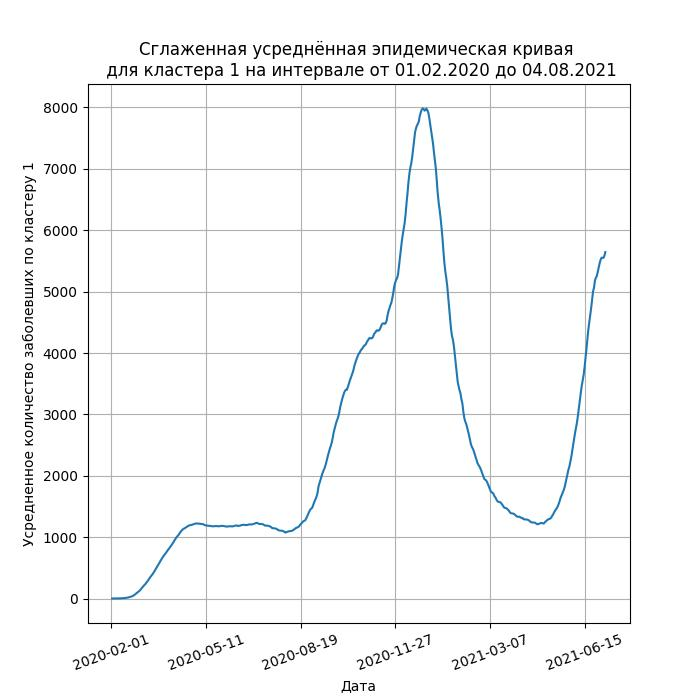
\includegraphics[width=0.5\textwidth]{../figures/clasters1.jpg}
	\caption{Sample figure caption.}
	\label{fig:fig1}
\end{figure}


В кластер 2 вошли Австрия, Германия, Италия, Сербия, Болгария, Румыния, Северная Македония, Венгрия, Иордания, Польша, Украина, Канада, Республика Молдова, Сирия, Босния и Герцеговина, Норвегия, Финляндия, Албания, Эстония, Черногория, Ливан, Словакия, Чехия, Азербайджан, Литва, Хорватия, Грузия, Дания, Беларусь, Латвия, Словения, Нидерланды, Армения, Люксембург, Бельгия, Кения, Швейцария, Швеция, Палестина.
Страны, вошедшие в кластер 2 географически локализованы главным образом в Европе. Из рисунка \ref{fig:fig2} видно существование двух выраженных пиков на интервале с октября 2020г. до
мая 2021 г.

\begin{figure}
	\centering
	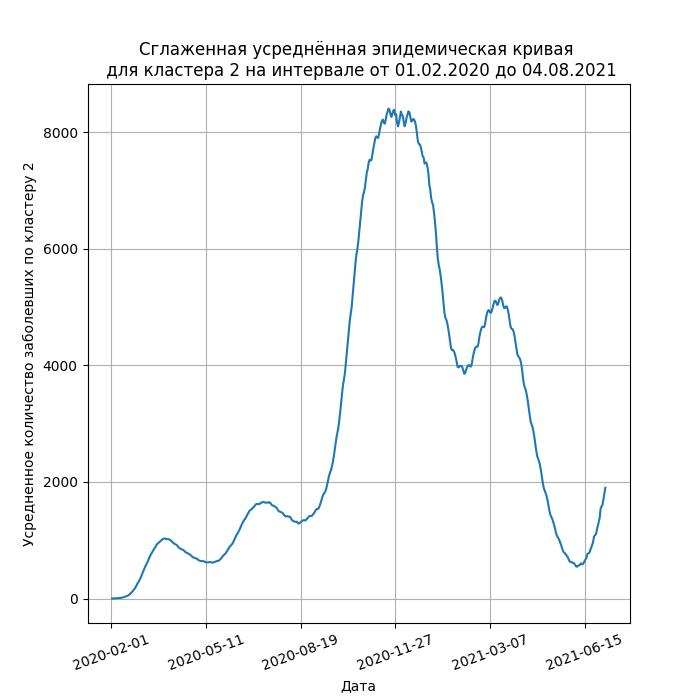
\includegraphics[width=0.5\textwidth]{../figures/clasters2.jpg}
	\caption{Sample figure caption.}
	\label{fig:fig2}
\end{figure}


В кластер 3 вошли Алжир, Марокко, Бангладеш, Вьетнам, Индонезия, Куба, Малайзия, Таиланд, Лаос, Мьянма, Тунис, Ливия, Греция, Иран, Кипр, Япония, Республика Корея. Кластер 3 содержит преимущественно страны с тропическим климатом. Сглаженная усреднённая эпидемическая кривая для кластера 3 приведены на рисунке \ref{fig:fig3}.

\begin{figure}
	\centering
	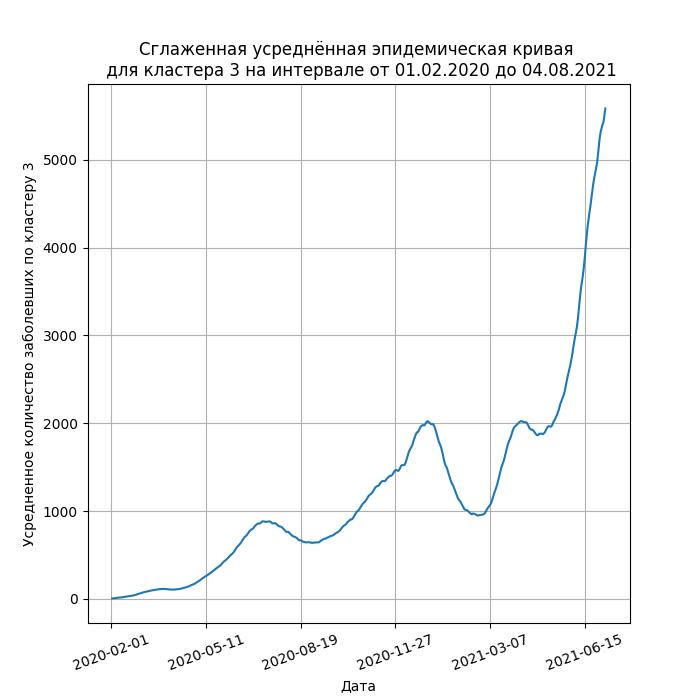
\includegraphics[width=0.5\textwidth]{../figures/clasters3.jpg}
	\caption{Sample figure caption.}
	\label{fig:fig3}
\end{figure}

В кластер 4 вошли Аргентина, Колумбия, Парагвай, Уругвай, Камбоджа, Шри Ланка, Бразилия, Ирак, Кувейт, Филиппины, Индия, Непал, Монголия. Значительная часть стран из кластера 4 географически локализована в Южной Америки. Из рисунка \ref{fig:fig4} можно отметить высокую интенсивность эпидемии с апреля 2020 г. по август 2021 г.

\begin{figure}
	\centering
	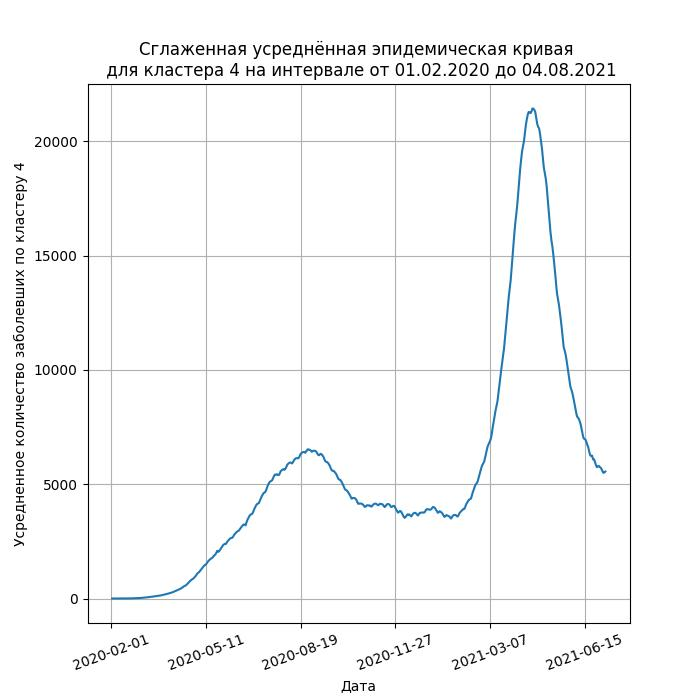
\includegraphics[width=0.5\textwidth]{../figures/clasters4.jpg}
	\caption{Sample figure caption.}
	\label{fig:fig4}
\end{figure}

В число стран, вошедших в мелкие кластеры или не образовавших кластеров вообще вошли Катар, Саудовская Аравия, Сингапур, Таджикистан. Боливия, Египет, Чили, Гватемала, Коста Рика, Оман, Мадагаскар, Перу, Эфиопия, Казахстан, Турция, Австралия, Гонду-
рас, Исландия, Испания, Йемен, Кыргызстан, Китай, Никарагуа, Новая Зеландия, Пакистан, Судан, Танзания, Узбекистан, Франция, Эквадор.

Для данных о динамике заболеваемости за временной промежуток от 22-01-2020 до 05-08-2021 среднее значение всех вычисленных силуэтов при разделении стран на 4 обозначенных
кластера составило 0.36.

Для верификации результата предлагается вычислить коэффициент с помощью использования перестановок. Полученные коэффициенты корреляции мы будем переставлять симметрично относительно диагонали в исходной матрице, содержащей все возможные лаговые корреляции. Осуществим 5000 различных перестановок $f$ и посчитаем коэффициенты силуэта. Максимальное значение коэффициента силуэта равно −0.02.

Проведем кластеризацию для случайных сгенерированных временных рядов из нормаль-
ного распределения. Значения в полученной таблице максимальных лаговых корреляций между сгенерированными рядами не превышали корреляцию равную 0.22. В связи с этим для сгенерированных временных рядов выберем точку останова равную 0.8 для прекращения слияния кластеров. Выбор нового порога основан на медианном значение полученных лаговых корреляций. Полученный коэффициент силуэта на основе алгоритма 3 для нашей кластеризации составил -0.004. Не смотря на отрицательное значение коэффициента силуэта он все же остается выше, чем коэффициенты для полученных перестановок - максимальный коэффициент силуэта для 5000 перестановок составил -0.005.


\section{Вывод}
В работе описан метод кластеризации временных рядов, приведен способ оценки значимости кластеризации. В ходе экспериментов показана хорошая работа на эпидемиологических кривых Covid-19. В дальнейшем планируется усовершенствовать метод кластеризации с помощью введения остановки слияния кластеров в заыисимости от вычисляемых $\rho$-значений для каждого кластера на каждом этапе слияния. 




\bibliographystyle{unsrtnat}
\bibliography{references}

\end{document}
